% !TEX root = ../my-thesis.tex
%
\chapter{Introduction}
\label{sec:intro}
\section{Background}
Controlling or even trying to prevent an infectious disease is a challenging task, and therefore it is crucial to find ways to combat this type of disease through new and creative ways. The number of infections can vary greatly between different countries or regions, and it is therefore of great interest for local governments or health institutes to find the underlying factors for these differences. This may lead to the identification of previously unrecognised environmental factors that could be the cause of the different risk of disease in different areas. One of the earliest examples of this type of analysis was carried out in relation to a cholera outbreak in south London in 1854 by John Snow. By creating the map shown in Figure~\ref{cholera}, he was able to show that cholera cases occurred mainly around a water pump in Broad Street. These findings were crucial to understanding that cholera spread through contaminated water supplies, and thus led to the modernisation of water supply and sanitation systems in London and the rest of the world \autocite[][]{snow1857cholera}.
\begin{figure}[H]
    \centering
    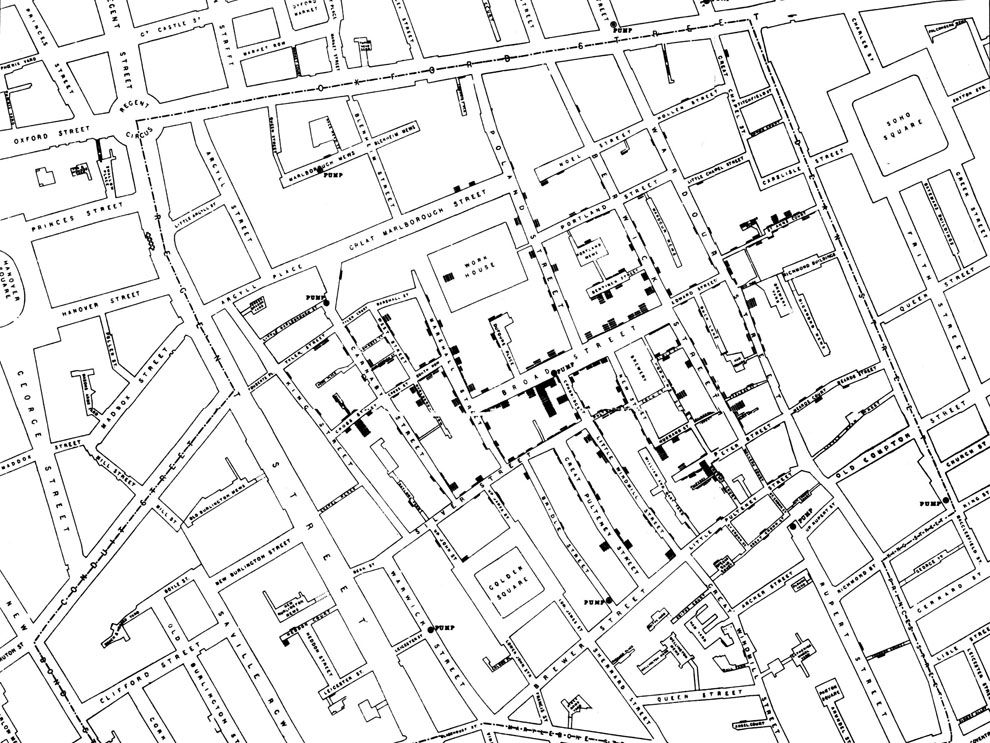
\includegraphics[width = 0.75\textwidth]{cholera_map.jpg}
    \caption{The original map of cholera cases in southern London, created by John Snow in 1854.}
    \label{cholera}
\end{figure}
The location itself (that is, a set of geographic coordinates) is generally unlikely to influence the risk of a certain disease; as there is no reason why one set of coordinates would inherently be at higher risk than another. Instead, the geographic location is a proxy measure, for differences in the attributes of the areas. These differences may relate to physical geography (e.g. temperature, sunlight, precipitation), environmental factors (e.g. air pollution, water quality) or population attributes(e.g. age, income, migration background). The identification of disparities in disease risk across a geographic region can lead to further investigation of the underlying reasons for the differences, which can lead to health breakthroughs such as those noted by Snow. Furthermore, by identifying areas of high risk, health authorities can focus additional resources on these areas in an attempt to influence the behaviours of the population that contribute to an increased risk of disease. \\
Most approaches to disease mapping are based on dividing the geographic region into spatial units, with disease risks estimated for each of these units. The reason for this is that individual-level data would violate patient confidentiality and governments are more interested in risk levels for the entire population. Each spatial unit has different demographics, so comparisons between spatial units are generally based on the standardised incidence ratio (SIR), defined as the number of observed cases in a given area divided by the number of cases expected for that area based on its population demographics.  Most modern methodology for estimating disease risk relies on conditional autoregressive (CAR) models \autocite[][]{besag1991bayesian}, which assume the existence of spatial autocorrelation between neighbouring areas, based on the notion that nearby areas are more likely to have more in common than areas that are further apart. This is due to the fact that adjacent areas are more likely to have similar socio-economic characteristics in terms of deprivation and population behaviour. It is assumed by these models that this level of spatial autocorrelation is constant across the spatial region.
\clearpage
\section{Motivation}
Covid-19 has had a significant impact on the lives of probably almost everyone on earth. Whether people had to work from home, children suddenly had online classes or people just stayed at home more, everyone was affected. Everyone had to get used to this new reality where suddenly you couldn't meet for a coffee or go to the cinema together because those establishments were either closed or people had no desire to risk contracting Covid-19. And that, of course, says nothing about the impact it had on the lives of people who became infected with Covid-19 or had relatives who became infected. The point is that everyone was affected by the impact of the pandemic, and still is, albeit at different levels. \\
Over time, different countries introduced different strategies to combat Covid-19, such as hard lockdowns where people were only allowed to leave the house if they had a legitimate reason to do so, for example to go to work or to buy groceries, while other countries did not introduce any lockdown measures. Other measures included wearing face masks in public places or limiting how many people can meet in public and private spaces. But even when the same measures were implemented in one country, there were big differences between the proportion of infected people in different parts of the country. \\
Finally, attitudes towards these measures have become a matter of political identity in various countries, as political parties from different spectrums have different views on how this pandemic should be handled, what measures should be implemented, or whether this pandemic even exists or if it is just much ado about nothing. This has also led to the formation of new political movements that regularly protest against the measures taken by the government and demand a return to pre-pandemic conditions. \\
Understanding the reason why the number of infections varies in different parts of the country can be crucial in helping local governments decide which measures to implement to limit the risk of infection and contribute to the common goal of ending the pandemic as soon as possible. \\
Identifying areas where people are at higher risk of becoming infected can also help governments decide on vaccination strategies, as it may make more sense to vaccinate people in high-risk areas first. By limiting the number of infections in these areas, the likelihood of the virus spreading from one of these areas to one or more neighbouring areas decreases, which in turn slows the spread of Coronavirus.
\clearpage
\section{Aim and Objective}
The main objective of this thesis is to analyse which factors drive the infection numbers of Covid-19 and thus increase the risk of people becoming infected and falling ill with the virus. To answer this question, a basic concept of Bayesian theory and Bayesian spatial models is developed and an introduction to geospatial data and the analysis of this specific type of data is given. For the analysis, different types of data need to be collected from different sources. The type of data includes
\begin{itemize}
    \item Data related to the number of infections in a given municipality.
    \item Data related to the number of vaccinations in a given municipality.
    \item Demographic data related to a specific municipality.
    \item Data related to spatial points of interest in a given municipality.
    \item Shapefiles for the geographic areas of interest.
\end{itemize}
In the analysis, these data are collected for two countries, Germany and Norway. These two countries are not equally affected by the pandemic and the population is distributed differently in the two countries, which makes for an interesting comparison of what factors influence the infection numbers and what kind of models work well in each country.\
In order to achieve the main objective of this thesis, there are the following important goals:
\begin{itemize}
    \item[1.] Build a basic concept of Bayesian theory and analysis of geospatial health data.
    \item[2.] Collect all the data needed for the analysis.
    \begin{itemize}
    \item[2.1] Collect data related to Covid-19 from the National Institutes of Health.
    \item[2.2] Collect demographic data and shapefiles from other official sources.
    \item[2.3] Collect infrastructure data by querying OpenStreetMap.
    \end{itemize}
    \item[3.] Merge all data from different sources to create a clean dataset for analysis.
    \item[4.] Develop and compare different types of Bayesian spatial models.
    \item[5.] Critically evaluate the models.
    \item[6.] Extract factors that significantly influence the risk of infection.
\end{itemize}
\clearpage
\section{Corona Virus}
\label{sec:corona}
Viral diseases continue to pose a serious public health threat. Several viral epidemics have occurred in the last 20 years, including the SARS pandemic in 2002/3, H1N1 influenza in 2009, and more recently the Middle East Respiratory Syndrome Coronavirus (MERS-CoV), which was first detected in Saudi Arabia in 2012. \\
In late 2019, the first few cases of lower respiratory infections were detected in Wuhan, China. In February 2020, this viral disease was officially named "Covid-19", an acronym for "Coronavirus Disease 2019". \\
Due to the rapid spread of the virus, a Public Health Emergency of International Concern was declared at the end of January 2020, with 18 countries reporting cases and four countries reporting human-to-human transmission. \\
At the end of February 2020, the World Health Organisation (WHO) raised the risk of a Covid 19 epidemic to "very high" before declaring it a pandemic on 11 March. At that time, more than 118,000 cases in 114 countries and 4000 deaths had already been registered. \\
The first cases of the disease were linked to direct exposure at the Huanan Seafood Wholesale Market in Wuhan, with animal-to-human transmission suspected as the main mechanism. After subsequent cases could not be linked to this mechanism, human-to-human transmission was presumed to be the main transmission mechanism. Furthermore, sympotomatic individuals are thought to be the most common source of Covid-19 spread. However, asymptomatic individuals can also transmit the virus, therefore isolation is the best way to contain this epidemic. \\
Similar to other respiratory diseases, e.g. influenza, transmission is thought to occur through respiratory droplets (particles $>5-10\mu m$ in diameter) when coughing and sneezing. In closed rooms, transmission by aerosol is also possible. \\
Based on the data from the first cases in Wuhan, the incubation period is generally between 3 and 7 days, with a median of 5.1 days. According to the data, the number of infections doubled about every seven days and the basic reproductive number $R$ is 2.2, which means that on average each infected individual infects another 2.2 individuals. \\
According to a report by the Chinese Centre for Disease Control, which studied 72,314 cases, the overall mortality rate of confirmed cases was 2.3\%, with most of the fatal cases affecting people over 70 years of age. \\
Furthermore, the clinical manifestations of the disease can be divided into three groups according to their severity:
\begin{itemize}
    \item Mild disease: non-pneumonia and mild pneumonia; this occurred in 81\% of cases.
    \item Severe disease: dyspnea, respiratory rate $\geq 30$ min, blood oxygen level $\leq 93\%$; this occurred in 14\% of cases.
    \item Critical disease: respiratory failure, septic shock and/or multiple organ dysfunction or failure; this occurred in 5\% of cases.
\end{itemize}
Subsequent reports indicate that the disease is asymptomatic or with very mild symptoms in 70\% of patients, while the remaining 30\% develop a respiratory syndrome with high fever, cough and even severe respiratory failure, which may require admission to the intensive care unit. \\
Most countries use some kind of clinical and epidemiological information to determine who should be tested. A molecular test, for example a PCR test, can be used to detect the disease.\\
The WHO recommends the collection of samples from both the upper and lower respiratory tract. In the laboratory, the genetic material extracted from the saliva or mucus sample is amplified by reverse polymerase chain reaction (RT-PCR), which synthesises a double-stranded DNA molecule from an RNA form. Once the genetic material is sufficient, the parts of the genetic code of the CoV that are conserved are searched for. The probes used are based on the original gene sequence published by the Shanghai Public Health Clinical Center \& School of Public Health, Fudan University, Shanghai, China on Virological.org and subsequent confirmatory evaluation by other laboratories \autocite[][]{cascella2021features}.
\clearpage
\section{Related Work and Contribution}
Since the start of the pandemic in 2019, numerous scientific papers have been written on Covid-19, covering a wide range of topics, such as medicine, social sciences and statistics. Naturally, there have also been papers written on the relationship between geographic regions and Covid-19. Incorporating a spatial dimension into the research process can help to better understand different phenomena and make them potentially mappable. The papers considered here can be divided into two categories. The first group consists of disease mapping, spatial analysis and spatio-temporal analysis and refers to studies that analyse the spatial and spatio-temporal patterns of Covid-19. The other group contains research that focuses on other factors that influence the dynamics of the Covid-19 pandemic, but may also include spatial and spatio-temporal analysis.
\subsection*{Disease Mapping, Spatial Analysis and Spatio-Temporal Analysis}
Guan et al. (2020) studied cases in mainland China up to 25 February 2020 to determine the defining clinical features and severity of the disease. Among other things, they found that Covid-19 spread rapidly throughout the country and that the severity of the disease varied. Furthermore, they found that the most common symptoms experienced by patients were cough and fever. They reported a median incubation period of 4 days \autocite[][]{guan2020clinical}. \\
Chen et al. (2020) analysed how people who emigrated from Wuhan contributed to the early stages of the pandemic in China at the beginning of 2020. They found a strong correlation between the number of confirmed cases of Covid-19 in a given province and emigration from Wuhan. They also found that the lockdown of several cities in Hubei province and the implementation of nationwide control measures were effective in preventing the exponential growth of the number of cases \autocite[][]{chen2020distribution}. \\
Similar to this study, Gross et al. (2020) compare the infection rate in different cities in China and provinces in Italy during the early phases of the pandemic and conclude that the spread of the disease is defined by a two-stage process. The first stage, the authors say, is defined by a constant rate of infection due to a lack of means to detect infected individuals before symptoms appear. In the second stage, they observed an approximately exponential decline due to quarantine. While they found differences between China and Italy, most notably that it took longer for outbreaks of the disease to be controlled in the Italian provinces, they found similar behaviour in terms of infection rate \autocite[][]{gross2020spatio}. \\
Chen et al. (2021) analysed the spatio-temporal distribution characteristics and influencing factors of the virus in mainland China using statistical methods, correlation analyses and geographic information system (GIS) mapping. They concluded that the outbreak in non-Hubei provinces can be divided into five phases. The initial outbreak phase, the peak phase where the highest number of new infections is observed, the containment phase where the number of new infections decreases, the rebound phase and a final phase where the number of new infections flattens out. They also observed that cities with large population flows from Wuhan were more affected by Covid-19 \autocite[][]{chen2021spatio}. \\
Saha et al. (2020) provide an overview of how GIS, e.g. mapping dashboards and applications, can be used to monitor the pandemic and related activities. They conclude that the pandemic requires massive data generation and GIS to enable rapid response and analysis to help prevent and guide decisions and movements \autocite[][]{saha2020monitoring}. \\
Gianquintieri et al. (2020) used geo-referenced calls to the emergency number relevant to respiratory problems and subsequent emergency medical service interventions to derive an unbiased representation of Covid-19 diffusion. This study was conducted for the Lombardy region of Italy, which was particularly hard hit by the pandemic in early 2020. The authors reported a strong correlation between Covid-19-related deaths at the provincial level and emergency calls and age- and sex-weighted ambulance dispatches \autocite[][]{gianquintieri2020mapping}. \\
Lastly, Petrov et al. (2020) examined the spatio-temporal dynamics of the pandemic in the Arctic up to July 2020. They found that the number of infections and morbidity were highly variable, but generally below national levels. They classified the Arctic regions into four groups: Iceland, the Faroe Islands, northern Norway and northern Finland, which were characterised by increased early infection rates but containment of the pandemic through quarantine and other measures; Northern Sweden and Alaska, where the first wave of infection persisted despite weak (Sweden) or variable (Alaska) quarantine measures; northern Russia, where a late start led to a steep rise in infections, deaths and several outbreaks; and northern Canada and Greenland where there was no significant spread of the pandemic \autocite[][]{petrov2020spatiotemporal}.
\subsection*{Other Factors Influencing the Pandemic}
Xiong et al. (2020) carried out a correlation analysis for the number of cases in the Hubei province between 30 January 2020 and 18 February 2020. They found a significant correlation between population, regional GDP , retail sales of consumer goods and the number of confirmed cases of Covid-19 in Hubei province, among others \autocite[][]{xiong2020spatial}. \\
Ahmadi et al. (2020) analysed the influence of climatic factors on the spread of Covid-19 in Iran and found that areas with low wind speed, humidity and solar radiation support the survival of the virus. The same study also found a direct correlation between population density and movement within provinces \autocite[][]{ahmadi2020investigation}. Mehmood et al. (2021) analysed the relationship between air pollution, climate, socioeconomic factors and infection rates in Pakistan. They reported a significant positive correlation between particulate matter $\left(\hbox{PM}_{2.5}\right)$, an air pollutant, and the number of infections. In contrast to Ahmadi et al. the correlation between the factors humidity and wind speed and the number of infections was positive in some regions and negative in others. They also found a small negative relationship between population density and Covid-19 cases, suggesting that areas with higher population density reported proportionally fewer cases \autocite[][]{mehmood2021spatiotemporal}. \\
Pedrosa (2020) analysed the relationship between the number of cases in the US and weather, demographic variables and the infection timeline. He found that only population density and a time series variable, defined as the number of days between the first and the 100th case, showed statistical significance, while the climate in the USA had no influence on infection numbers \autocite[][]{pedrosa2020dynamics} \\
As the United States is one of the countries most affected by the pandemic, many studies have attempted to determine what factors are driving up the number of infections in the country. Mollalo et al. (2020) analysed the spatial variability of Covid-19 in the United States up to the 9th of April 2020. Out of 35 environmental, socio-economic, topographical and demographic variables, the four variables found to be most significant were: income inequality, median household income, the proportion of black females and the proportion of nurse practitioners at the county level \autocite[][]{mollalo2020gis}. \\
Maiti et al. (2021) analysed infection counts up to 13 May 2020 in the USA. They observed a higher risk of Covid-19 clusters in metropolitan areas compared to rural counties, counties near central airports, more populous counties and counties with the highest proportion of racial and ethnic minorities \autocite[][]{maiti2021exploring}. \\
Wang et al. (2021) analysed the numbers up to 29 January 2021 in the US and find that factors of ethnicity, crime and income have positive correlations with the number of Covid-19 cases and explain most of the variance in the modelling estimate \autocite[][]{wang2021spatiotemporal}. \\
Allcott et al. (2020) examine partisan differences in Americans' responses to the Covid-19 pandemic, specifically how Republicans and Democrats socially distance themselves and make other efforts to reduce transmission of the disease. They model not the risk of being infected, but how a person's political beliefs affect their beliefs about the Covid-19 pandemic. They find significant individual-level differences between Republicans and Democrats in self-reported social distancing, beliefs about their personal risk of being infected, and beliefs about the future severity of the pandemic. According to the study, Democrats find it significantly more important to stay inside to prevent the spread of the virus than to go outside to help the economy, compared to Republicans \autocite[][]{allcott2020polarization}. \\
Bermudi et al. (2021) modelled mortality in the country using latent Gaussian-Bayesian spatial models and found significant relationships between Covid-19 mortality and socioeconomic conditions, as higher socioeconomic levels, as measured by a socioeconomic index, were shown to lead to a lower risk of mortality due to Covid-19. In addition, they showed that men and older persons had the highest risk of mortality due to Covid-19 \autocite[][]{bermudi2021spatiotemporal}. Castro et al (2020), on the other hand, could not find a single narrative that explains the spread of the virus across the states of Brazil, but rather found that layers of complex scenarios intertwine, resulting in a different and simultaneous Covid 19 epidemic across Brazil \autocite[][]{castro2021spatiotemporal}. \\
The situation in India was analysed in a paper by Nandy et al. (2021) and the authors found that higher investment in health and education reduced the likelihood of the spread of Covid-19. In addition, a higher cure rate was found in states with sustained investment in health and education, with mortality rates also lower in states that invest more in education \autocite[][]{nandy2021managing}. \\
Sannigrahi et al. (2020) found a significant correlation between selected demographic and socio-economic components, including total population, poverty and income, and the number of deaths from Covid-19 in Europe, without controlling for other factors such as environmental variables, socio-ecological status or climate extremes\autocite[][]{sannigrahi2020examining}. \\
Studies have also been conducted analysing the impact of interdiction measures on the spread of Covid-19. Kasilingam et al. (2020) attempted to predict early containment of Covid-19 using machine learning models based on infrastructural and environmental variables, as well as government-implemented policies and infection-related independent variables for 42 countries. Using logistic regression, a significant positive association was found between healthcare infrastructure and lockdown policies and signs of early containment \autocite[][]{kasilingam2020exploring}.
Orea and Álvarez (2020) also found a significant positive relationship between interdiction in Spain and its usefulness in preventing the spread of Covid-19 between different provinces in Spain. Furthermore, the same type of relationship was found for the spread of Covid-19 within the same province \autocite[][]{orea2020effective}. \\
\subsection*{Contribution}
The information contained in all the papers mentioned earlier shows just how many different factors may or may not be associated with the way that Coronavirus spreads in different countries. Finding a perfect model that explains why numbers are higher in one geographical region than in another is utopian, as there are still too many unknowns even more than a year into the pandemic. Achieving a scientific breakthrough is therefore beyond the scope of this work, the aim is rather to consider a wide range of factors, including infrastructural factors, demographic and socio-economic variables, when discussing the reason for different infection figures within a country and between two different countries. The countries selected for this work, Norway and Germany, are not equally affected by Covid-19, so looking for factors that influence infection numbers in both countries may be indicative of a variable that is driving infection numbers up or down, independent of the country.
\clearpage
\section{Thesis Outline}
The structure of the thesis is as follows. First, an introduction to Bayesian inference is given in Chapter~\ref{sec:bayes}. This part includes basic concepts of Bayesian theory, e.g. Bayes' theorem, which are essential for the methodology used in this thesis. Furthermore, different types of priors are introduced, as they form an integral part in Bayesian modelling. In addition, Markov-chain-Monte-Carlo-methods (MCMC methods) and latent Gaussian models are introduced, the latter of which can overcome the shortcomings of MCMC methods and form the basis for Bayesian spatial models. The last part of this chapter includes the introduction of goodness-of-fit indicators used to evaluate model performance and addresses some problems of Bayesian spatial models. \\
In Chapter~\ref{sec:geodata} a brief introduction to the analysis of geospatial health data is given. First, different types of geospatial data, namely vector data and raster data, are introduced before discussing different methodologies used in modelling this type of data. These methodologies include the standardised incidence ratio (SIR) and the estimation of disease risk in spatial areas. \\
Chapter~\ref{sec:datacollection} gives a brief overview of the different types of data collected in this thesis and how the different data sources were combined into a coherent dataset. Chapter~\ref{sec:analysis} then shows how these data were analysed. This includes calculating the SIR for Norway and Germany and modelling the relationships between different variables of interest and infection numbers in these countries. Two classes of models were calculated for this purpose: Models without a spatial component and models with such a component. Finally, an analysis is carried out to see how the results of the analysis change when different priors are used.